%% abtex2-modelo-trabalho-academico.tex, v-1.9.2 laurocesar
%% Copyright 2012-2014 by abnTeX2 group at http://abntex2.googlecode.com/ 
%%
%% This work may be distributed and/or modified under the
%% conditions of the LaTeX Project Public License, either version 1.3
%% of this license or (at your option) any later version.
%% The latest version of this license is in
%%   http://www.latex-project.org/lppl.txt
%% and version 1.3 or later is part of all distributions of LaTeX
%% version 2005/12/01 or later.
%%
%% This work has the LPPL maintenance status `maintained'.
%% 
%% The Current Maintainer of this work is the abnTeX2 team, led
%% by Lauro César Araujo. Further information are available on 
%% http://abntex2.googlecode.com/
%%
%% This work consists of the files abntex2-modelo-trabalho-academico.tex,
%% abntex2-modelo-include-comandos and abntex2-modelo-references.bib
%%

% ------------------------------------------------------------------------
% ------------------------------------------------------------------------
% abnTeX2: Modelo de Trabalho Academico (tese de doutorado, dissertacao de
% mestrado e trabalhos monograficos em geral) em conformidade com 
% ABNT NBR 14724:2011: Informacao e documentacao - Trabalhos academicos -
% Apresentacao
% ------------------------------------------------------------------------
% ------------------------------------------------------------------------

\documentclass[
	% -- opções da classe memoir --
	12pt,				% tamanho da fonte
	openright,			% capítulos começam em pág ímpar (insere página vazia caso preciso)
	oneside,			% para impressão em verso e anverso. Oposto a oneside
	a4paper,			% tamanho do papel. 
	% -- opções da classe abntex2 --
	%chapter=TITLE,		% títulos de capítulos convertidos em letras maiúsculas
	%section=TITLE,		% títulos de seções convertidos em letras maiúsculas
	%subsection=TITLE,	% títulos de subseções convertidos em letras maiúsculas
	%subsubsection=TITLE,% títulos de subsubseções convertidos em letras maiúsculas
	% -- opções do pacote babel --
	english,			% idioma adicional para hifenização
	french,				% idioma adicional para hifenização
	spanish,			% idioma adicional para hifenização
	brazil				% o último idioma é o principal do documento
	]{abntex2}

% ---
% Pacotes básicos 
% ---
\usepackage{xcolor}
\definecolor{verde}{rgb}{0.25,0.5,0.35}
\definecolor{jpurple}{rgb}{0.5,0,0.35}
\usepackage{lmodern}			% Usa a fonte Latin Modern			
\usepackage[T1]{fontenc}		% Selecao de codigos de fonte.
\usepackage[utf8]{inputenc}		% Codificacao do documento (conversão automática dos acentos)
\usepackage{lastpage}			% Usado pela Ficha catalográfica
\usepackage{indentfirst}		% Indenta o primeiro parágrafo de cada seção.
\usepackage{color}				% Controle das cores
\usepackage{graphicx}			% Inclusão de gráficos
\usepackage{microtype} 			% para melhorias de justificação
\usepackage{listings}
\lstset{
  language=Java,
  basicstyle=\ttfamily\small, 
  keywordstyle=\color{jpurple}\bfseries,
  stringstyle=\color{red},
  commentstyle=\color{verde},
  morecomment=[s][\color{blue}]{/**}{*/},
  extendedchars=true, 
  showspaces=false, 
  showstringspaces=false, 
  numbers=left,
  numberstyle=\tiny,
  breaklines=true, 
  backgroundcolor=\color{cyan!10}, 
  breakautoindent=true, 
  captionpos=b,
  xleftmargin=0pt,
  tabsize=4
}
% ---
		
% ---
% Pacotes adicionais, usados apenas no âmbito do Modelo Canônico do abnteX2
% ---
\usepackage{lipsum}				% para geração de dummy text
% ---

% ---
% Pacotes de citações
% ---
\usepackage[brazilian,hyperpageref]{backref}	 % Paginas com as citações na bibl
\usepackage[alf]{abntex2cite}	% Citações padrão ABNT

% --- 
% CONFIGURAÇÕES DE PACOTES
% --- 
\newcommand\tab[1][1cm]{\hspace*{#1}}
\setlength\afterchapskip{\lineskip} %espaçamento entre capítulo e texto, que diminuiu este espaço. Entretanto, não sei se é o espaço exigido pela universidade
\setlength\aftersecskip{\lineskip}	%espaçamento entre seção e texto
\setlength\aftersubsecskip{\lineskip} %espaçamento entre subseção e texto
% ---
% Configurações do pacote backref
% Usado sem a opção hyperpageref de backref
% ---

% ---
% Informações de dados para CAPA e FOLHA DE ROSTO
% ---
\titulo{Linguagem de Programação JAVA}
\autor{Gabriel Campos,Luigi Soares,Vinicius Carvalho,Matheus Possas}
\local{Belo Horizonte - Brasil}
\data{2018}
% O preambulo deve conter o tipo do trabalho, o objetivo, 
% o nome da instituição e a área de concentração 
\preambulo{Trabalho Teórico Prático apresentado na disciplina de Linguagens de Programação do curso de Ciência da Computação da Pontifícia Universidade Católica de Minas Gerais sobre a linguagem de programação JAVA.
.}
% ---


% ---
% Configurações de aparência do PDF final

% alterando o aspecto da cor azul
\definecolor{blue}{RGB}{41,5,195}

% informações do PDF
\makeatletter
\hypersetup{
     	%pagebackref=true,
		pdftitle={\@title}, 
		pdfauthor={\@author},
    	pdfsubject={\imprimirpreambulo},
	    pdfcreator={LaTeX with abnTeX2},
		pdfkeywords={abnt}{latex}{abntex}{abntex2}{trabalho acadêmico}, 
		colorlinks=true,       		% false: boxed links; true: colored links
    	linkcolor=blue,          	% color of internal links
    	citecolor=blue,        		% color of links to bibliography
    	filecolor=magenta,      		% color of file links
		urlcolor=blue,
		bookmarksdepth=4
}
\makeatother
% --- 

% --- 
% Espaçamentos entre linhas e parágrafos 
% --- 

% O tamanho do parágrafo é dado por:
\setlength{\parindent}{1.3cm}

% Controle do espaçamento entre um parágrafo e outro:
\setlength{\parskip}{0.2cm}  % tente também \onelineskip

% ---
% compila o indice
% ---
\makeindex
% ---

% ----
% Início do documento
% ----
\begin{document}

% Retira espaço extra obsoleto entre as frases.
\frenchspacing 

% ----------------------------------------------------------
% ELEMENTOS PRÉ-TEXTUAIS
% ----------------------------------------------------------
% \pretextual

% ---
% Capa
% ---
\imprimircapa

% ---

% ---
% Folha de rosto
% (o * indica que haverá a ficha bibliográfica)
% ---
\imprimirfolhaderosto*

% ---


% ---
% inserir lista de ilustrações
% ---
\pdfbookmark[0]{\listfigurename}{lof}
\listoffigures*
\cleardoublepage
% ---

% ---
% inserir lista de tabelas
% ---
%\pdfbookmark[0]{\listtablename}{lot}
%\listoftables*
%\cleardoublepage
% ---

% ---
% inserir o sumario
% ---
\pdfbookmark[0]{\contentsname}{toc}
\tableofcontents*

% ---



% ----------------------------------------------------------
% ELEMENTOS TEXTUAIS
% ----------------------------------------------------------
\textual

% ----------------------------------------------------------
% Introdução (exemplo de capítulo sem numeração, mas presente no Sumário)
% ----------------------------------------------------------
\chapter[Introdução]{Introdução}
%\addcontentsline{toc}{chapter}{Introdução}

Java é uma linguagem de programação interpretada de alto nível orientada a objetos
e plataforma de software. 9 milhões de desenvolvedores criaram aplicações Java em várias
indústrias de ponta.
Diferente das linguagens de programação convencionais, que são compiladas para
código nativo, a linguagem Java é compilada para um código binário que é interpretado por
uma máquina virtual.
Os dois principais componentes da plataforma Java são a Java Application
Programming Interface (API), que é a biblioteca de linhas de comando do Java, e a Java
Virtual Machine (JVM), que interpreta o código Java em linguagem de máquina.

% ----------------------------------------------------------
{\let\clearpage\relax \chapter[Histórico]{Histórico}}
%\chapter[Histórico]{Histórico}
%\addcontentsline{toc}{chapter}{Histórico}


Em 1991, o Green Project foi iniciado, na Sun Microsystems, o início do Java,
uma linguagem de programação orientada a objetos. Os líderes do
projeto eram Patrick Naughton, Mike Sheridan, e James Gosling. O projeto tinha como objetivo antecipar e planejar o próximo passo do mundo digital, e não a criação de uma nova linguagem de programação.

Eles acreditavam que em algum tempo haveria uma maior integração dos computadores com os equipamentos e eletrodomésticos bastante utilizados pelas pessoas em casa e no trabalho durante o cotidiano. Para validar a viabilidade desta idéia, treze pessoas trabalharam arduamente durante 18 meses. No segundo semestre de 1992, a equipe fez emergir de um escritório de Sand Hill Road, no Menlo Park, uma demonstração funcional da idéia inicial. 

O protótipo se chamava *7 (leia-se “StarSeven”, ou “Estrela Sete” em português), um
controle remoto com uma interface gráfica utilizando a tecnologia de tela sensível ao toque. Para o *7 foi criado um mascote, hoje amplamente conhecido no mundo Java, o Duke.

\begin{figure}[!h]
\centering
  
\includegraphics[width=0.3\linewidth]{Java-duke.jpg}
  \caption{Mascote Java}
  \label{fig:Mascote Java}
\end{figure}


Duke no *7 era ser um guia virtual, ajudando e ensinando o usuário a utilizar o equipamento. O *7 tinha a capacidade de controlar diversos dispositivos e aplicações. James Gosling especificou uma nova linguagem de programação para o *7. Gosling decidiu batizá-la de “Oak”, que quer dizer “carvalho”, uma árvore que ele podia observar quando olhava pela sua janela. 

O próximo passo era encontrar um mercado para o *7. A equipe achava que uma boa idéia seria controlar televisores e vídeo por demanda com o equipamento. Eles construíram um demo chamado MovieWood, mas infelizmente era muito cedo para que o vídeo por demanda bem como as empresas de TV a cabo pudessem viabilizar o negócio, pois o custo era alto demais e a infraestrutura era escassa. 

Hoje em dia, já é realidade em programas interativos e também na televisão digital, porém a ideia do *7 na época não emplacou.  Permitir ao telespectador interagir com a emissora e com a programação em uma grande rede cabos, era algo muito visionário e estava muito longe do que as empresas de TV a cabo tinham capacidade de entender e comprar. A idéia certa, na época errada.

Com a alta da Internet, rapidamente uma grande rede interativa estava se estabelecendo; Era este tipo de rede interativa que a equipe do *7 estava tentando vender para as empresas de TV a cabo. E, em poucos meses, não era mais necessário construir a infra-estrutura para a rede, ela simplesmente estava lá. Gosling foi incumbido de adaptar o Oak para a Internet e, em janeiro de 1995, foi lançada uma nova versão do Oak rebatizada para Java. 

\begin{figure}[!h]
\centering
  
\includegraphics[width=0.75\linewidth]{java.jpg}
  \caption{Simbolo Java}
  \label{fig:Mascote Java}
\end{figure}

A tecnologia Java tinha sido projetada para se expandir por meio das redes de dispositivos heterogêneos, redes como a Internet. Agora aplicações poderiam ser
executadas dentro dos Browsers nos Applets Java e tudo seria disponibilizado pela Internet de forma instantânea. Foi o HTML estático dos Browsers que promoveu a rápida disseminação da tecnologia Java. A velocidade dos acontecimentos seguintes foi tremenda, o número de usuários cresceu rapidamente, grandes empresas do ramo, como a IBM anunciaram suporte para a tecnologia Java.

Desde seu lançamento, em maio de 1995, a plataforma Java foi adotada mais rapidamente do que qualquer outra linguagem de programação na história da computação. Em 2003 Java atingiu a marca de 4 milhões de desenvolvedores em todo mundo. Java continuou e continua crescendo e hoje é com certeza um padrão para o mercado oferecendo qualidade, performance e segurança ainda sem nenhum competidor a altura. Java tornou-se popular pelo seu uso na Internet e hoje possui seu ambiente de execução presente em web browsers, mainframes, SOs, celulares, palmtops
e cartões inteligentes, entre outros.

Em 2008 a Oracle Corporation adquire a empresa responsável pela linguagem Java, a Sun Microsystems, por US\$ 7,4 bilhões, com o objetivo de levar o Java e outros produtos da Sun ao dispor dos consumidores.

O Java foi influenciado pela linguagens C/C++ pela sua sintaxe. E influenciou o javascript, as duas linguagens possuem suporte à programação funcional.

\section{Versões do Java}

Desde o lançamento do Java, vêm surgindo várias versões e alterações nas nomenclaturas e conteúdos. Abaixo é apresentada uma linha do tempo referente às evoluções das versões que formaram a linguagem Java:

\subsection{Java Development Kit (JDK ou Java 1.0)}

Criada no ano de 1996.
É a 1ª versão sendo hoje usada para compatibilidade de browsers mais antigos;

\subsection{Java Development Kit (JDK ou Java 1.1)}

Criada no ano de 1997.
Obteve muitas bibliotecas adicionadas das quais se destacaram o Java RMI, JavaBeans, novo modelo de eventos, JDBC (driver para conexão com banco de dados).

\subsection{Java Standard Edition (J2SE 1.2 ou Java 2)}

Criada no ano de 1998.
Grande aumento das classes na biblioteca Java (API), ficando considerada a versão da mudança do nome para as versões do produto (JDK) e também sendo optada pela divisão de 3 tipos de plataformas. O principal motivo para essa ação foi que muitos desenvolvedores e usuários estavam confundindo a linguagem Java da linguagem Javascript, que são diferentes. A partir daqui todas as versões Java foram denominadas de Java 2 Standard Edition, que passaram a ter apelidos ou codinomes, esta versão ficou conhecida como Playground da qual foi adicionado o Framework Collections entre outros.

\subsection{Java Standard Edition - J2SE 1.3}

Criada no ano de 2000.
Codinome Kestrel, inclusão das bibliotecas JNDI, JavaSound entre outros.


\subsection{Java Standard Edition J2SE 1.4}

Criada no ano de 2002.
Codinome Merlin, criada a palavra reservada “assert”, biblioteca NIO entre outros.


\subsection{Java Standard Edition J2SE 5.0}

Criada no ano de 2004.
A versão mais usada, sendo conhecida com o codinome Tiger. Apesar da versão ser 1.5, agora é chamada apenas de 5. Adições importantes como: Enumeração, Autoboxing, Generics, for-each entre outros estão nela.


\subsection{Java Standard Edition JSE 6}

Criada no ano de 2006.
Codinome Mustang, teve outras alterações que mudaram na nomenclatura (remoção do 2 - J2SE) e melhora significativa na performance e na estabilidade tendo o surgimento do JIT.


\subsection{Java Standard Edition JSE 7 }
Criada no ano de 2011.
Suporte ao uso de strings em condições do switch.
Inferência na criação de objetos com tipos genéricos.
Simplificação na invocação de métodos com parâmetros varargs e tipos genéricos.
Gerenciamento automático de recursos, tais como conexões a bancos de dados, I/O.
Possibilidade de tratar diversas exceções em um mesmo catch (Multicatch) entre outros.

\subsection{Java Standard Edition JSE 8 }

Java 8 é a release mais recente do Java, porém em fase de testes, disponível apenas para desenvolvedores.
Possui métodos de expressão Lambda e Extensão virtual além de API de Data e Hora.

Uma nova implementação leve de alto desempenho do motor JavaScript foi integrada ao JDK, a Nashhorn JavaScript Engine.


\section{Linguagens Similares}

\subsection{Semelhança em Orientação à objetos}

As linguagens a seguir tem semelhança com Java em orientação por objetos: VB.NET, Object Pascal, Objective-C, Python, SuperCollider, Ruby, Smalltalk, C\#, C++.

\subsection{Semelhança Imperativa}

As linguagens a seguir tem semelhança com Java por causa de seu paradigma Imperativo: Ada, ALGOL, Basic, C, PHP, Cobol, Fortran, Pascal, Python, Lua, Mathematica.

\subsection{Semelhança funcional}

A partir da versão 8, o Java adiciona aspectos de linguagem funcional, permitindo utilizar técnicas funcionais, como mapeamento, redução, bem como tratar funções como variáveis, para isso são utilizadas interfaces para esse tipo de manipulação.
As linguagens a seguir tem semelhança em Java por causa de seu paradigma funcional: APL, Lisp, ML, Haskell, OCaml, F\#, Elixir.



{\let\clearpage\relax \chapter[Paradigma]{Paradigma}}
%\addcontentsline{toc}{chapter}{Paradigma}

Java é uma linguagem de programação multiparadigma, isto é, ela é baseada em mais de um paradigma ao mesmo tempo. Temos a orientação à objetos, programação imperativa e funcional como seus principais paradigmas.

Linguagens OO(orietada à objetos) descrevem as iterações entre os objetos. Um objeto é formado por estados e funcionamento. Os estados é representados por dados e o funcionamento por funções, que atuam no objeto em questão. Linguagens OO também manipulam os dados de entrada para gerar de dados de saída específicos, e cada objeto tem uma funcionalidade diferente.

No Java todos os objetos são auto-sufiencietes, isto é todos os seus modulos são inerentemente reutilizáveis. Podemos também adicionar novos procedimentos e
subclasses a qualquer objeto.

Para o paradigma imperativo, podemos pensar que ele transforma a computação em ações, assemelhando-se com o comportamento das linguagens naturais que expressam ordens.
Tal paradigma também pode ser chamado de paradigma procedural, e a forma que este paradigma funciona é baseada em comandos, porque o intuito era ser parecido com a linguagem de maquina.

Java também é funcional, o que pode ser um pouco estranho já que é imperativo, porém é uma linguagem que consegue diferenciar bem os paradigmas de sua computação.
A ideia do paradigma funcional é de avaliar funções matematicas e o java serve muito bem para este proposito, como realizar calculos de volumes e areas de funções trigonometricas.

Os demais paradigmas são: estruturado, genérico, reflectivo e concorrente.

{\let\clearpage\relax \chapter[Características]{Características}}
%\addcontentsline{toc}{chapter}{Características}

Java é uma linguagem simples em sua especificação, tanto da linguagem em si
como do ambiente de execução (JVM), é distribuída com um vasto conjunto de bibliotecas
(ou APIs), suporta nativamente caracteres Unicode, possui facilidades para criação de
programas distribuídos e multitarefa (múltiplas linhas de execução num mesmo programa) e
desalocação de memória automática por um processo conhecido como coletor de lixo.

Confiabilidade: O processo de compilação elimina vários possíveis problemas e a
checagem dinâmica (em tempo de execução) contorna várias situações que poderiam gerar
erros. Essas situações, chamas exceções, podem ser devidamente tratadas para evitar que
o programa aborte.

Segurança: Um programa sempre é verificado antes de ser executado, e como a
linguagem não permite acesso direto à memória, impede seu uso para o desenvolvimento
de vírus.

Portabilidade: Um programa em Java não depende de uma plataforma específica, é
possível executá-lo em qualquer lugar.

Recursos de Rede: Java possui uma extensa biblioteca de rotinas, que facilitam a
cooperação com protocolos TCP/IP, como HTTP e FTP.

\section{Método Main}
O método main é onde o programa inicia. Ele pode estar presente em qualquer classe.
Os parâmetros de linha de comando são enviados para o array de Strings chamado args.

\begin{lstlisting}
public static void main(String[] args) {
	// Corpo da main
}
\end{lstlisting}
\section{Classes}

Uma classe é um elemento do código Java que utilizamos para representar objetos
do mundo real. Dentro dela é comum declararmos atributos e métodos, que representam,
respectivamente, as características e comportamentos desse objeto.

\begin{lstlisting}
class Carro{ 
	// Corpo da classe
}
\end{lstlisting}

É possível especificar o modificador de acesso da classe de forma a determinar sua
visibilidade. Pode ser public, private ou protected.

\begin{lstlisting}
public Class Moto {
	// Corpo da classe
}
\end{lstlisting}

Programas em Java são formados por uma coleção de classes armazenadas
independentemente e que podem ser carregadas no momento de utilização.
Java implementa os conceitos de orientação à objetos como abstração,
encapsulamento, polimorfismo e herança.

\begin{lstlisting}
Class Automovel {
	public void acelerar() {
		// Corpo do metodo
	}
	public void abastecer() {
		// Corpo do metodo
	}
}
Class Carro extends Automovel {
	@Override
	public void acelerar() {
		motor();
	}
	public void abastecer() {
		// Corpo do metodo
	}
	private void motor() {
		// Corpo do metodo
	}
}
\end{lstlisting}
Java não suporta herança múltipla, devido à possibilidade de uma classe pai ter um
método com o mesmo nome de outra classe pai, e gerar possíveis falhas ao chamar o
método, e todas as classes em Java derivam da classe Object. A única possibilidade de se
ver herança múltipla em Java é no uso de interfaces, pois uma classe pode implementar
várias interfaces.

\section{Estruturas}

\subsection{“Condicional”}

Exemplo da estrutura "If/Else" em Java:
\begin{lstlisting}
if(<condicao>){ 
	//Condicao verdadeira
}else{
	//Condicao falsa
}
\end{lstlisting}

Outra estrutura condicional bastante utilizada é o "Switch/case":

\begin{lstlisting}
switch (numero inteiro % 2){
	case 0:
		System.out.println("Numero Par");
		break;
	case 1:
		System.out.println("Numero Impar");
		break;
	default:
		break;
}
\end{lstlisting}

\subsection{“Repetição”}

Existem 3 maneiras de utilizar uma estrutura de repetição em Java, "For","While", "Do while". O exemplo a seguir mostra a estrutura "For":

\begin{lstlisting}
for(int i = 0;i < 10;i++){ 
	<linha de codigo a ser repetida 10 vezes>
} 
\end{lstlisting}

\subsection{“Tabela unidimensional”}

Exemplo da criação de uma tabela unidimensional em Java:

\begin{lstlisting}
public static void main(String[]args){ 
	int[] array = new int[<tamanho da tabela>];
}
\end{lstlisting}

\subsection{“Chamada de função”}

Exemplo de uma chamada de função em Java:

\begin{lstlisting}
public static void main(String[]args){ 
	int a = 1;int b = 5;
	int c  = soma(a,b);
}
public int soma(int a,int b)\{ 
	int x;
	x = a+b;
	return x;
}
\end{lstlisting}

\subsection{“Tratamento Exceção”}

Em caso de erro de compilação, erros devem ser tratados, uma boa maneira de tratá-los é usando Tratamento de Exceção. Segue um exemplo de Tratamento de Exceção:

\begin{lstlisting}
try{ 
	//Trecho de codigo ao qual deve ser tratado
	... (codigo)
	throw new tipoExcecao(e);
    ... (codigo)
}catch(Exception e){ 
	//possiveis acoes e mensagens de erro
}
\end{lstlisting}


\subsection{“Arquivo”}
Exemplo de Arquivos em Java:

\begin{lstlisting}
File arquivo = new File("texto.txt");
if(!arquivo.exists()){
	System.out.println("O arquivo nao existe");
}
\end{lstlisting}

\section{\textit{Interface}}

Uma interface modela um comportamento esperado. Pode-se entendê-la como uma
classe que contenha apenas métodos abstratos. Embora uma classe não possa conter mais
de uma superclasse, a classe pode implementar mais de uma interface.

\begin{lstlisting}
public interface Combustao {
	void queimarGasolina();
	void queimarAlcool();
}
Class Automovel {
	public void acelerar() {
		// Corpo do metodo
	}
	public void abastecer() {
		// Corpo do metodo
	}
}
Class Carro extends Automovel implements Combustao {
	@Override
	public void acelerar() {
		motor();
	}
	public void abastecer() {
		// Corpo do metodo
	}
	private void motor() {
		queimarGasolina();
	}
	private void queimarGasolina() {
		// Corpo do metodo
	}
	private void queimarAlcool() {
		// Corpo do metodo
	}
}
\end{lstlisting}

\section{Objetos Anônimos}

\begin{lstlisting}
public Class Poluicao {
	public static void main(String[] args) {
		// Nao e necessario instanciar o objeto em uma variavel para utiliza-lo:
		new Carro().acelerar();
	}
}
\end{lstlisting}

\section{Coletor de lixo}

O coletor de lixo (garbage collector) é um processo usado para a automação do
gerenciamento de memória. Com ele é possível recuperar uma área de memória inutilizada,
como uma instância de um objeto que não será mais utilizada no programa, desalocando
então a área de memória reservada para aquela instância, o que pode evitar problemas de
vazamento de memória, resultando no esgotamento da memória livre para alocação.

\section{Arcabouços}

Um arcabouço, também conhecido como framework, é uma abstração que une
códigos comuns entre vários projetos de software provendo uma funcionalidade genérica.
São utilizados para facilitar o desenvolvimento de aplicações. Os mais utilizados são:
Hibernate, Junit, Log4g, Spring e Struts.

\section{Ambientes de desenvolvimento}

IDE, do inglês Integrated Development Environment ou Ambiente de
Desenvolvimento Integrado, é um programa que reúne ferramentas necessárias para o
desenvolvimento de aplicações de software, como um editor, compilador, depurador e
outros. Algumas IDEs mais conhecidas e utilizadas para o desenvolvimento de aplicações
em Java são: Eclipse, Netbeans, JGRASP e IntelliJ IDEA.

{\let\clearpage\relax \chapter[Exemplos]{Exemplos}}
%\addcontentsline{toc}{chapter}{Exemplos}

\section{Hello world!}
Exemplo mais basico das linguagens de programação,o "print" de um Hello world na tela.

\begin{lstlisting}
public static void main(String[] args) {
	System.out.println("Hello World!");
}
\end{lstlisting}

\section{Calculo Lambda}

Exemplo de Calculo Lambda em Java.

\begin{figure}[!h]
\centering
  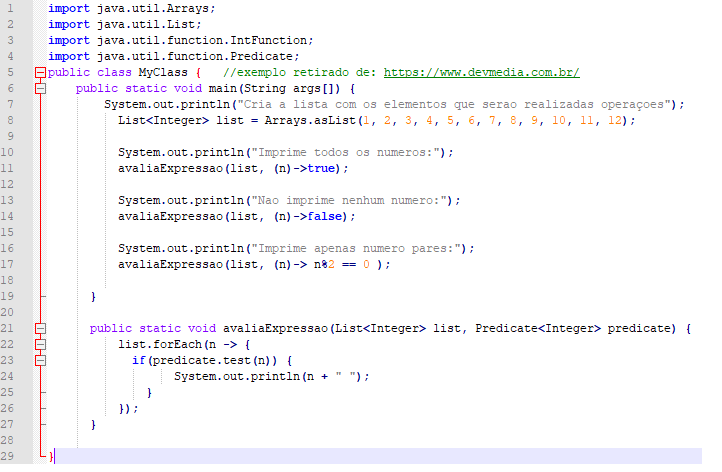
\includegraphics[width=0.8\linewidth]{calculoLmb.png}
  \caption{Calculo Lambda}
  \label{fig:Calc}
\end{figure}



\section{Forma Escalonada Reduzida}

Exemplo de uma matriz sendo modificada para sua Forma Escalonada Reduzida, com a finalidade de achar a matriz identidade.

\begin{figure}[!h]
\centering
  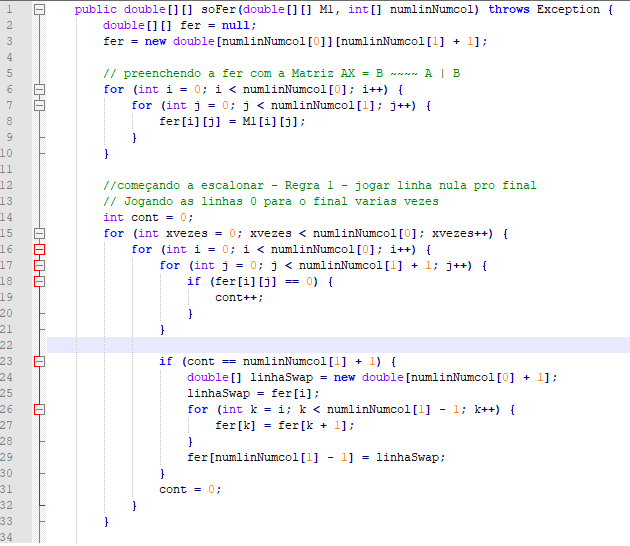
\includegraphics[width=0.95\linewidth]{fer1.png}
\end{figure}

\begin{figure}[!h]
\centering
  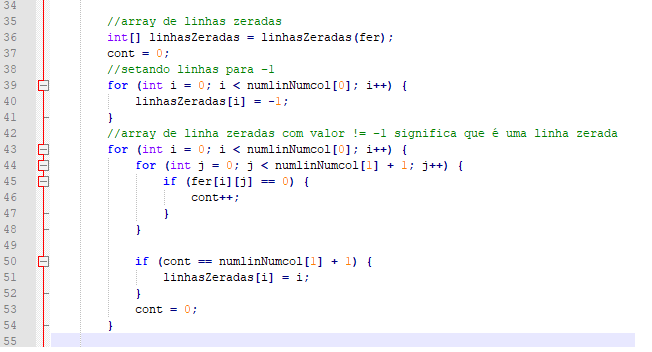
\includegraphics[width=0.95\linewidth]{fer4.png}
\end{figure}

\begin{figure}[!h]
\centering
  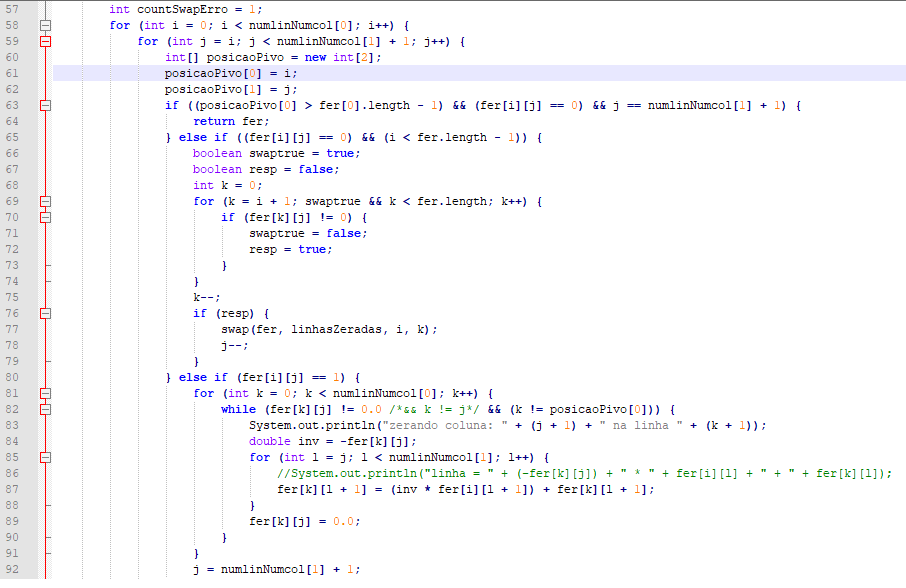
\includegraphics[width=0.83\linewidth]{fer3.png}
\end{figure}

\begin{figure}[!h]
\centering
  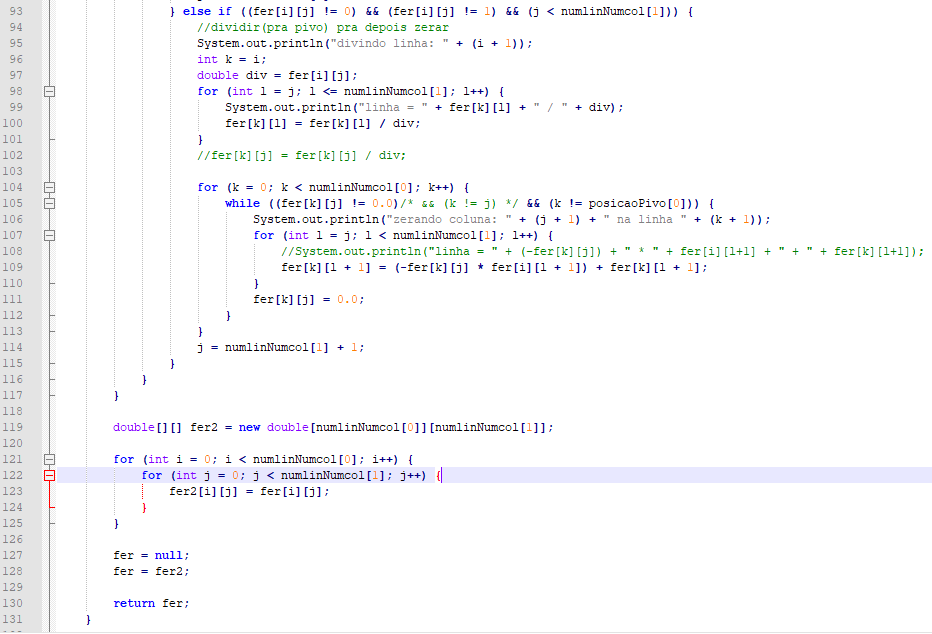
\includegraphics[width=0.83\linewidth]{fer2.png}
  \caption{Forma Escalonada Reduzida}
  \label{fig:Fer}
\end{figure}

% ---
% Conclusão (outro exemplo de capítulo sem numeração e presente no sumário)
% ---
{\let\clearpage\relax \chapter[Considerações Finais]{Considerações Finais}}
%\addcontentsline{toc}{chapter}{Considerações Finais}

Java é uma linguagem de programação atual com paradigma orientado à objetos, imperativa e funcional, sendo ela uma linguagem forte e estática, ela se destacou no mercado pela sua ampla plataforma, pois a mesma consegue programar não só para desktop, mas também para aplicativos celulares, cartões de banco, programação web e até televisão digital. Java também consegue programar não só em windows, mas também em Mac e GNU/Linux.
% ---


% ----------------------------------------------------------
% ELEMENTOS PÓS-TEXTUAIS
% ----------------------------------------------------------
\postextual
% ----------------------------------------------------------

% ----------------------------------------------------------
% Referências bibliográficas
% ----------------------------------------------------------
\nocite{100}
\nocite{101}
\nocite{1}
\nocite{2}
\nocite{3}
\nocite{4}
\nocite{5}
\nocite{6}
\nocite{7}
\nocite{8}
\nocite{9}
\nocite{10}

\bibliographystyle{unsrt}
\bibliography{referencia}
\end{document}
